\documentclass{article}




\usepackage{fullpage}
\usepackage{nopageno}
\usepackage{amsmath}
\usepackage{amsfonts}
\usepackage{graphicx}
\usepackage{framed}
\usepackage{algorithmic}
\usepackage{xcolor}

\definecolor{dark_red}{rgb}{0.5,0.0,0.0}
\definecolor{dark_green}{rgb}{0.0,0.5,0.0}
\definecolor{dark_blue}{rgb}{0.0,0.0,0.5}
\definecolor{blue}{rgb}{0.0,0.0,1.0}

\newcommand{\dr}[1]{\textcolor{dark_red}{#1}}
\newcommand{\dg}[1]{\textcolor{dark_green}{#1}}
\newcommand{\db}[1]{\textcolor{dark_blue}{#1}}
\newcommand{\blue}[1]{\textcolor{blue}{#1}}



\begin{document}

\section*{Orthogonality}

Consider the set of \(n\) component vectors \(\mathbb{R}^n\). 

\[\|\mathbf{u}\| = \left\|\begin{bmatrix} u_1 \\ u_2 \\ \vdots \\ u_n \end{bmatrix}\right\| = \sqrt{u_1^2 + u_2^2 + ... + u_n^2}\]

\[\mathbf{u} \bullet \mathbf{v} = \begin{bmatrix} u_1 \\ u_2 \\ \vdots \\ u_n \end{bmatrix} \bullet \begin{bmatrix} v_1 \\ v_2 \\ \vdots \\ v_n \end{bmatrix} = u_1 v_1 + u_2 v_2 + ... + u_n v_n\]

Note that \(\|\mathbf{u}\| = \sqrt{\mathbf{u} \bullet \mathbf{u}}\). 

\(\mathbf{u} \bullet \mathbf{v} = 0\) if and only if \(\mathbf{u}\) and \(\mathbf{v}\) are perpendicular, also referred to as being orthogonal.

Given a set of \(k\) vectors \(A = \{\mathbf{u}_1, \mathbf{u}_2, ..., \mathbf{u}_k\}\), \(A\) is {\bf orthogonal} if and only if \(\mathbf{u}_i \bullet \mathbf{u}_j = 0\) for all \(i \neq j\). If it is also the case that every vector from \(A\) has a magnitude of \(1\), then \(A\) is {\bf orthonormal}.



\subsection*{Determining orthogonality}

A set of \(k\) vectors \(A = \{\mathbf{u}_1, \mathbf{u}_2, ..., \mathbf{u}_k\}\), \(A\) is {\bf orthogonal} if and only if \(\mathbf{u}_i \bullet \mathbf{u}_j = 0\) for all \(i \neq j\). This condition can be directly tested using an \(n \times k\) matrix \(B\) where the vectors from \(A\) form the columns of \(B\):

\[B = \begin{bmatrix} \mathbf{u}_1 & \mathbf{u}_2 & \cdots & \mathbf{u}_k \end{bmatrix}\]

It is then the case that:

\[B^T B 
= \begin{bmatrix} \mathbf{u}_1^T \\ \mathbf{u}_2^T \\ \vdots \\ \mathbf{u}_k^T \end{bmatrix}\begin{bmatrix} \mathbf{u}_1 & \mathbf{u}_2 & \cdots & \mathbf{u}_k \end{bmatrix}
= \begin{bmatrix} \mathbf{u}_1^T \mathbf{u}_1 & \mathbf{u}_1^T \mathbf{u}_2 & \cdots & \mathbf{u}_1^T \mathbf{u}_k \\
\mathbf{u}_2^T \mathbf{u}_1 & \mathbf{u}_2^T \mathbf{u}_2 & \cdots & \mathbf{u}_2^T \mathbf{u}_k \\
\vdots & \vdots & \ddots & \vdots \\
\mathbf{u}_k^T \mathbf{u}_1 & \mathbf{u}_k^T \mathbf{u}_2 & \cdots & \mathbf{u}_k^T \mathbf{u}_k \end{bmatrix} 
= \begin{bmatrix} \mathbf{u}_1 \bullet \mathbf{u}_1 & \mathbf{u}_1 \bullet \mathbf{u}_2 & \cdots & \mathbf{u}_1 \bullet \mathbf{u}_k \\
\mathbf{u}_2 \bullet \mathbf{u}_1 & \mathbf{u}_2 \bullet \mathbf{u}_2 & \cdots & \mathbf{u}_2 \bullet \mathbf{u}_k \\
\vdots & \vdots & \ddots & \vdots \\
\mathbf{u}_k \bullet \mathbf{u}_1 & \mathbf{u}_k \bullet \mathbf{u}_2 & \cdots & \mathbf{u}_k \bullet \mathbf{u}_k \end{bmatrix} \]

If \(A\) is an orthogonal set of vectors, then all non diagonal entries of \(B^T B\) should be \(0\). If \(A\) additionally contains no zero vectors, then the diagonal entries of \(B^T B\) are all nonzero. If \(A\) is an orthonormal set of vectors, then \(B^T B\) is the \(k \times k\) identity matrix \(B^T B = I\). 


\vspace{5mm}

If \(A = \{\mathbf{u}_1, \mathbf{u}_2, ..., \mathbf{u}_n\}\) is an orthogonal set of \(n\) nonzero vectors, then the \(n \times n\) matrix \(B\): 

\[B = \begin{bmatrix} \mathbf{u}_1 & \mathbf{u}_2 & \cdots & \mathbf{u}_k \end{bmatrix}\]

has the following inverse:

\[B^{-1} = \begin{bmatrix} \frac{1}{\mathbf{u}_1 \bullet \mathbf{u}_1}\mathbf{u}_1^T \\ \frac{1}{\mathbf{u}_2 \bullet \mathbf{u}_2}\mathbf{u}_2^T \\ \vdots \\ \frac{1}{\mathbf{u}_n \bullet \mathbf{u}_n}\mathbf{u}_n^T \end{bmatrix}\]


\vspace{5mm}

If \(A = \{\mathbf{u}_1, \mathbf{u}_2, ..., \mathbf{u}_n\}\) is an orthonormal set of \(n\) vectors, then the \(n \times n\) matrix \(B\): 

\[B = \begin{bmatrix} \mathbf{u}_1 & \mathbf{u}_2 & \cdots & \mathbf{u}_n \end{bmatrix}\]

has the following inverse:

\[B^{-1} = B^T = \begin{bmatrix} \mathbf{u}_1^T \\ \mathbf{u}_2^T \\ \vdots \\ \mathbf{u}_n^T \end{bmatrix}\]


\vspace{5mm}

In general, if an orthogonal set does not contain any zero vectors, then the set is linearly independent and is hence a basis for its span.


\vspace{5mm}

\textbf{Examples:}*
\begin{itemize}
%%%%%%%%%%%%%%%%%%%%%%%%%%%
\item Given the set of vectors \(A = \left\{\mathbf{u}_1 = \begin{bmatrix} 1 \\ 0 \\ -1 \end{bmatrix}, \mathbf{u}_2 = \begin{bmatrix} 2 \\ 0 \\ 2 \end{bmatrix}, \mathbf{u}_3 = \begin{bmatrix} 0 \\ 5 \\ 0 \end{bmatrix}\right\}\), let \(B = \begin{bmatrix} \mathbf{u}_1 & \mathbf{u}_2 & \mathbf{u}_3 \end{bmatrix} = \begin{bmatrix} 1 & 2 & 0 \\ 0 & 0 & 5 \\ -1 & 2 & 0 \end{bmatrix}\). 
\[B^T B = \begin{bmatrix} 1 & 0 & -1 \\ 2 & 0 & 2 \\ 0 & 5 & 0 \end{bmatrix}\begin{bmatrix} 1 & 2 & 0 \\ 0 & 0 & 5 \\ -1 & 2 & 0 \end{bmatrix} = \begin{bmatrix} 2 & 0 & 0 \\ 0 & 8 & 0 \\ 0 & 0 & 25 \end{bmatrix}\]
\(B^T B\) is diagonal, so the vectors in set \(A\) are orthogonal. \(B^T B \neq I\) however so the vectors in set \(A\) are not orthonormal however. Since no vectors in set \(A\) are zero, matrix \(B\) is invertible and has the inverse:
\[B^{-1} = \begin{bmatrix} 1/2 & 0 & -1/2 \\ 1/4 & 0 & 1/4 \\ 0 & 1/5 & 0 \end{bmatrix}\]
%%%%%%%%%%%%%%%%%%%%%%%%%%%
\item Given the set of vectors \(A = \left\{\mathbf{u}_1 = \begin{bmatrix} 1/5 \\ 1/5 \\ 1/5 \end{bmatrix}, \mathbf{u}_2 = \begin{bmatrix} -1/2 \\ 1/2 \\ 0 \end{bmatrix}, \mathbf{u}_3 = \begin{bmatrix} 1/3 \\ 1/3 \\ -2/3 \end{bmatrix}\right\}\), let \(B = \begin{bmatrix} \mathbf{u}_1 & \mathbf{u}_2 & \mathbf{u}_3 \end{bmatrix} = \begin{bmatrix} 1/5 & -1/2 & 1/3 \\ 1/5 & 1/2 & 1/3 \\ 1/5 & 0 & -2/3 \end{bmatrix}\). 
\[B^T B = \begin{bmatrix} 1/5 & 1/5 & 1/5 \\ -1/2 & 1/2 & 0 \\ 1/3 & 1/3 & -2/3 \end{bmatrix}\begin{bmatrix} 1/5 & -1/2 & 1/3 \\ 1/5 & 1/2 & 1/3 \\ 1/5 & 0 & -2/3 \end{bmatrix} = \begin{bmatrix} 3/25 & 0 & 0 \\ 0 & 1/2 & 0 \\ 0 & 0 & 2/3 \end{bmatrix}\]
\(B^T B\) is diagonal, so the vectors in set \(A\) are orthogonal. \(B^T B \neq I\) however so the vectors in set \(A\) are not orthonormal however. Since no vectors in set \(A\) are zero, matrix \(B\) is invertible and has the inverse:
\[B^{-1} = \begin{bmatrix} 5/3 & 5/3 & 5/3 \\ -1 & 1 & 0 \\ 1/2 & 1/2 & -1 \end{bmatrix}\]
%%%%%%%%%%%%%%%%%%%%%%%%%%%
\item Given the set of vectors \(A = \left\{\mathbf{u}_1 = \begin{bmatrix} -3/5 \\ 4/5 \\ 0 \end{bmatrix}, \mathbf{u}_2 = \begin{bmatrix} 4/5 \\ 3/5 \\ 0 \end{bmatrix}, \mathbf{u}_3 = \begin{bmatrix} 0 \\ 0 \\ 1 \end{bmatrix}\right\}\), let \(B = \begin{bmatrix} \mathbf{u}_1 & \mathbf{u}_2 & \mathbf{u}_3 \end{bmatrix} = \begin{bmatrix} -3/5 & 4/5 & 0 \\ 4/5 & 3/5 & 0 \\ 0 & 0 & 1 \end{bmatrix}\). 
\[B^T B = \begin{bmatrix} -3/5 & 4/5 & 0 \\ 4/5 & 3/5 & 0 \\ 0 & 0 & 1 \end{bmatrix}\begin{bmatrix} -3/5 & 4/5 & 0 \\ 4/5 & 3/5 & 0 \\ 0 & 0 & 1 \end{bmatrix} = \begin{bmatrix} 1 & 0 & 0 \\ 0 & 1 & 0 \\ 0 & 0 & 1 \end{bmatrix}\]
\(B^T B\) is diagonal, so the vectors in set \(A\) are orthogonal. Moreover, \(B^T B = I\) so the vectors in set \(A\) are also orthonormal. Matrix \(B\) is invertible and has the inverse:
\[B^{-1} = B^T = \begin{bmatrix} -3/5 & 4/5 & 0 \\ 4/5 & 3/5 & 0 \\ 0 & 0 & 1 \end{bmatrix}\]
\end{itemize}

*Examples from the problem set of chapter 6.3 of the textbook: \\
Anton, Howard; Rorres, Chris, \emph{Elementary Linear Algebra 11th edition, Applications Version}, Wiley, 2014.





\subsection*{Projections and perpendicular components}

Given a set of nonzero orthogonal vectors \(A = \{\mathbf{u}_1, \mathbf{u}_2, ..., \mathbf{u}_k\}\), the advantage of orthogonality is that there is an easy approach to determining the coefficients needed to express any vector from \(\text{span}(A)\) as a linear combination of the vectors from \(A\). 

Given any vector \(\mathbf{v}\) from the span of the orthogonal nonzero vectors \(\text{span}\{\mathbf{u}_1, \mathbf{u}_2, ..., \mathbf{u}_k\}\), the unique coefficients \(c_1\), \(c_2\), ..., \(c_k\) such that \(\mathbf{v} = c_1 \mathbf{u}_1 + c_2\mathbf{u}_2 + ... + c_k\mathbf{u}_k\) can be easily determined as follows:

Starting with 
\[c_1 \mathbf{u}_1 + c_2\mathbf{u}_2 + ... + c_k\mathbf{u}_k = \mathbf{v}\]
To find coefficient \(c_i\), multiply using the dot product both sides by \(\mathbf{u}_i\):
\begin{align*}
& c_1 \mathbf{u}_1 + c_2\mathbf{u}_2 + ... + c_k\mathbf{u}_k = \mathbf{v} \\
\implies & \mathbf{u}_i \bullet (c_1 \mathbf{u}_1 + ... + c_i\mathbf{u}_i + ... + c_k\mathbf{u}_k) = \mathbf{u}_i \bullet \mathbf{v} \\
\iff & c_1(\mathbf{u}_ i \bullet \mathbf{u}_1) + ... + c_i(\mathbf{u}_i \bullet \mathbf{u}_i) + ... + c_k(\mathbf{u}_i \bullet \mathbf{u}_k) = \mathbf{u}_i \bullet \mathbf{v} \\
\iff & c_1(0) + ... + c_i(\mathbf{u}_i \bullet \mathbf{u}_i) + ... + c_k(0) = \mathbf{u}_i \bullet \mathbf{v} \\
\iff & c_i(\mathbf{u}_i \bullet \mathbf{u}_i) = \mathbf{u}_i \bullet \mathbf{v} \\
\iff & c_i = \frac{\mathbf{u}_i \bullet \mathbf{v}}{\mathbf{u}_i \bullet \mathbf{u}_i}
\end{align*}

Vector \(\mathbf{v}\) can hence be expressed as the following linear combination:

\[\mathbf{v} = \frac{\mathbf{u}_1 \bullet \mathbf{v}}{\mathbf{u}_1 \bullet \mathbf{u}_1}\mathbf{u}_1 + \frac{\mathbf{u}_2 \bullet \mathbf{v}}{\mathbf{u}_2 \bullet \mathbf{u}_2}\mathbf{u}_2 + ... + \frac{\mathbf{u}_k \bullet \mathbf{v}}{\mathbf{u}_k \bullet \mathbf{u}_k}\mathbf{u}_k\]

For any vector \(\mathbf{v}\) (in the span or not) the linear combination:

\[\text{proj}(\mathbf{v} | \mathbf{u}_1, \mathbf{u}_2, ..., \mathbf{u}_k) = \frac{\mathbf{u}_1 \bullet \mathbf{v}}{\mathbf{u}_1 \bullet \mathbf{u}_1}\mathbf{u}_1 + \frac{\mathbf{u}_2 \bullet \mathbf{v}}{\mathbf{u}_2 \bullet \mathbf{u}_2}\mathbf{u}_2 + ... + \frac{\mathbf{u}_k \bullet \mathbf{v}}{\mathbf{u}_k \bullet \mathbf{u}_k}\mathbf{u}_k\]

is referred to as the ``projection" of \(\mathbf{v}\) onto the span of \(A\). The projection is equal to \(\mathbf{v}\) if and only if \(\mathbf{v}\) is in the span of \(A\), otherwise part of \(\mathbf{v}\), referred to as the ``perpendicular component" is removed by the projection.

The part of \(\mathbf{v}\) removed by the projection is:

\[\text{perp}(\mathbf{v} | \mathbf{u}_1, \mathbf{u}_2, ..., \mathbf{u}_k) = \mathbf{v} - \text{proj}(\mathbf{v} | \mathbf{u}_1, \mathbf{u}_2, ..., \mathbf{u}_k) = \mathbf{v} - \frac{\mathbf{u}_1 \bullet \mathbf{v}}{\mathbf{u}_1 \bullet \mathbf{u}_1}\mathbf{u}_1 - \frac{\mathbf{u}_2 \bullet \mathbf{v}}{\mathbf{u}_2 \bullet \mathbf{u}_2}\mathbf{u}_2 - ... - \frac{\mathbf{u}_k \bullet \mathbf{v}}{\mathbf{u}_k \bullet \mathbf{u}_k}\mathbf{u}_k\]

and is referred to as the ``perpendicular component" of \(\mathbf{v}\) relative to the span of \(A\). The perpendicular component is \(\mathbf{0}\) if and only if \(\mathbf{v}\) is in the span of \(A\).

\textbf{Examples:}*
\begin{itemize}
%%%%%%%%%%%%%%%%%%%%%%
\item Let \(\mathbf{u}_1 = \begin{bmatrix} 1/3 \\ 2/3 \\ -2/3 \end{bmatrix}\); \(\mathbf{u}_2 = \begin{bmatrix} 2/3 \\ 1/3 \\ 2/3 \end{bmatrix}\); and \(\mathbf{v} = \begin{bmatrix} 4 \\ 2 \\ 1 \end{bmatrix}\).

It can easily be checked that \(\mathbf{u}_1 \bullet \mathbf{u}_2 = 2/9 + 2/9 - 4/9 = 0\) so \(A = \{\mathbf{u}_1, \mathbf{u}_2\}\) is an orthogonal set. Computing the projection and perpendicular component of \(\mathbf{v}\) relative to the plane spanned by \(\mathbf{u}_1\) and \(\mathbf{u}_2\) is performed as follows. First compute:
\begin{itemize}
\item[*] \(\mathbf{u}_1 \bullet \mathbf{u}_1 = 1/9 + 4/9 + 4/9 = 1\)
\item[*] \(\mathbf{u}_2 \bullet \mathbf{u}_2 = 4/9 + 1/9 + 4/9 = 1\)
\item[*] \(\mathbf{u}_1 \bullet \mathbf{v} = 4/3 + 4/3 - 2/3 = 2\)
\item[*] \(\mathbf{u}_2 \bullet \mathbf{v} = 8/3 + 2/3 + 2/3 = 4\)
\end{itemize} 
so the projection is:
\begin{align*}
\text{proj}(\mathbf{v} | \mathbf{u}_1, \mathbf{u}_2) = & \frac{\mathbf{u}_1 \bullet \mathbf{v}}{\mathbf{u}_1 \bullet \mathbf{u}_1}\mathbf{u}_1 + \frac{\mathbf{u}_2 \bullet \mathbf{v}}{\mathbf{u}_2 \bullet \mathbf{u}_2}\mathbf{u}_2  
= \frac{2}{1}\begin{bmatrix} 1/3 \\ 2/3 \\ -2/3 \end{bmatrix} + \frac{4}{1}\begin{bmatrix} 2/3 \\ 1/3 \\ 2/3 \end{bmatrix} 
= \begin{bmatrix} 2/3 \\ 4/3 \\ -4/3 \end{bmatrix} + \begin{bmatrix} 8/3 \\ 4/3 \\ 8/3 \end{bmatrix} 
= \begin{bmatrix} 10/3 \\ 8/3 \\ 4/3 \end{bmatrix}
\end{align*}
and the perpendicular component is:
\[\text{perp}(\mathbf{v} | \mathbf{u}_1, \mathbf{u}_2) = \mathbf{v} - \text{proj}(\mathbf{v} | \mathbf{u}_1, \mathbf{u}_2) = \begin{bmatrix} 4 \\ 2 \\ 1 \end{bmatrix} - \begin{bmatrix} 10/3 \\ 8/3 \\ 4/3 \end{bmatrix} = \begin{bmatrix} 2/3 \\ -2/3 \\ -1/3 \end{bmatrix}\]
%%%%%%%%%%%%%%%%%%%%%%
\item Let \(\mathbf{u}_1 = \begin{bmatrix} 1 \\ -2 \\ 1 \end{bmatrix}\); \(\mathbf{u}_2 = \begin{bmatrix} 2 \\ 1 \\ 0 \end{bmatrix}\); and \(\mathbf{v} = \begin{bmatrix} 1 \\ 0 \\ 3 \end{bmatrix}\).

It can easily be checked that \(\mathbf{u}_1 \bullet \mathbf{u}_2 = 2 - 2 + 0 = 0\) so \(A = \{\mathbf{u}_1, \mathbf{u}_2\}\) is an orthogonal set. Computing the projection and perpendicular component of \(\mathbf{v}\) relative to the plane spanned by \(\mathbf{u}_1\) and \(\mathbf{u}_2\) is performed as follows. First compute:
\begin{itemize}
\item[*] \(\mathbf{u}_1 \bullet \mathbf{u}_1 = 1 + 4 + 1 = 6\)
\item[*] \(\mathbf{u}_2 \bullet \mathbf{u}_2 = 4 + 1 + 0 = 5\)
\item[*] \(\mathbf{u}_1 \bullet \mathbf{v} = 1 + 0 + 3 = 4\)
\item[*] \(\mathbf{u}_2 \bullet \mathbf{v} = 2 + 0 + 0 = 2\)
\end{itemize} 
so the projection is:
\begin{align*}
\text{proj}(\mathbf{v} | \mathbf{u}_1, \mathbf{u}_2) = & \frac{\mathbf{u}_1 \bullet \mathbf{v}}{\mathbf{u}_1 \bullet \mathbf{u}_1}\mathbf{u}_1 + \frac{\mathbf{u}_2 \bullet \mathbf{v}}{\mathbf{u}_2 \bullet \mathbf{u}_2}\mathbf{u}_2  
= \frac{4}{6}\begin{bmatrix} 1 \\ -2 \\ 1 \end{bmatrix} + \frac{2}{5}\begin{bmatrix} 2 \\ 1 \\ 0 \end{bmatrix} 
= \begin{bmatrix} 2/3 \\ -4/3 \\ 2/3 \end{bmatrix} + \begin{bmatrix} 4/5 \\ 2/5 \\ 0 \end{bmatrix} 
= \begin{bmatrix} 22/15 \\ -14/15 \\ 2/3 \end{bmatrix}
\end{align*}
and the perpendicular component is:
\[\text{perp}(\mathbf{v} | \mathbf{u}_1, \mathbf{u}_2) = \mathbf{v} - \text{proj}(\mathbf{v} | \mathbf{u}_1, \mathbf{u}_2) = \begin{bmatrix} 1 \\ 0 \\ 3 \end{bmatrix} - \begin{bmatrix} 22/15 \\ -14/15 \\ 2/3 \end{bmatrix} = \begin{bmatrix} -7/15 \\ 14/15 \\ 7/3 \end{bmatrix}\]
%%%%%%%%%%%%%%%%%%%%%%
\item Let \(\mathbf{u}_1 = \begin{bmatrix} 1 \\ 1 \\ 1 \\ 1 \end{bmatrix}\); \(\mathbf{u}_2 = \begin{bmatrix} 1 \\ 1 \\ -1 \\ -1 \end{bmatrix}\); and \(\mathbf{v} = \begin{bmatrix} 1 \\ 2 \\ 0 \\ -2 \end{bmatrix}\).

It can easily be checked that \(\mathbf{u}_1 \bullet \mathbf{u}_2 = 1 + 1 - 1 - 1 = 0\) so \(A = \{\mathbf{u}_1, \mathbf{u}_2\}\) is an orthogonal set. Computing the projection and perpendicular component of \(\mathbf{v}\) relative to the plane spanned by \(\mathbf{u}_1\) and \(\mathbf{u}_2\) is performed as follows. First compute:
\begin{itemize}
\item[*] \(\mathbf{u}_1 \bullet \mathbf{u}_1 = 1 + 1 + 1 + 1 = 4\)
\item[*] \(\mathbf{u}_2 \bullet \mathbf{u}_2 = 1 + 1 + 1 + 1 = 4\)
\item[*] \(\mathbf{u}_1 \bullet \mathbf{v} = 1 + 2 + 0 - 2 = 1\)
\item[*] \(\mathbf{u}_2 \bullet \mathbf{v} = 1 + 2 + 0 + 2 = 5\)
\end{itemize} 
so the projection is:
\begin{align*}
\text{proj}(\mathbf{v} | \mathbf{u}_1, \mathbf{u}_2) = & \frac{\mathbf{u}_1 \bullet \mathbf{v}}{\mathbf{u}_1 \bullet \mathbf{u}_1}\mathbf{u}_1 + \frac{\mathbf{u}_2 \bullet \mathbf{v}}{\mathbf{u}_2 \bullet \mathbf{u}_2}\mathbf{u}_2  
= \frac{1}{4}\begin{bmatrix} 1 \\ 1 \\ 1 \\ 1 \end{bmatrix} + \frac{5}{4}\begin{bmatrix} 1 \\ 1 \\ -1 \\ -1 \end{bmatrix} 
= \begin{bmatrix} 1/4 \\ 1/4 \\ 1/4 \\ 1/4 \end{bmatrix} + \begin{bmatrix} 5/4 \\ 5/4 \\ -5/4 \\ -5/4 \end{bmatrix} 
= \begin{bmatrix} 3/2 \\ 3/2 \\ -1 \\ -1 \end{bmatrix}
\end{align*}
and the perpendicular component is:
\[\text{perp}(\mathbf{v} | \mathbf{u}_1, \mathbf{u}_2) = \mathbf{v} - \text{proj}(\mathbf{v} | \mathbf{u}_1, \mathbf{u}_2) = \begin{bmatrix} 1 \\ 2 \\ 0 \\ -2 \end{bmatrix} - \begin{bmatrix} 3/2 \\ 3/2 \\ -1 \\ -1 \end{bmatrix} = \begin{bmatrix} -1/2 \\ 1/2 \\ 1 \\ -1 \end{bmatrix}\]
\end{itemize}

*Examples from the problem set of chapter 6.3 of the textbook: \\
Anton, Howard; Rorres, Chris, \emph{Elementary Linear Algebra 11th edition, Applications Version}, Wiley, 2014.




\section*{Gram-Schmidt orthogonalization}

Given an arbitrary linearly independent set of vectors \(A = \{\mathbf{v}_1, \mathbf{v}_2, ..., \mathbf{v}_k\}\), an orthogonal basis for \(\text{span}(A)\) can be derived by recursively eliminating from each vector the component that is parallel to the span of the previous vectors. Basis vector \(\mathbf{u}_i\) is derived from \(\mathbf{v}_i\) by computing the component of \(\mathbf{v}_i\) that is perpendicular to the span of the previous vectors: \(\mathbf{u}_i = \text{perp}(\mathbf{v}_i | \mathbf{u}_1, \mathbf{u}_2, ..., \mathbf{u}_{i-1})\)

\begin{align*}
\mathbf{u}_1 = & \mathbf{v}_1 \\  
\mathbf{u}_2 = & \text{perp}(\mathbf{v}_2 | \mathbf{u}_1) = \mathbf{v}_2 - \frac{\mathbf{u}_1 \bullet \mathbf{v}_2}{\mathbf{u}_1 \bullet \mathbf{u}_1}\mathbf{u}_1 \\  
\mathbf{u}_3 = & \text{perp}(\mathbf{v}_3 | \mathbf{u}_1, \mathbf{u}_2) = \mathbf{v}_3 - \frac{\mathbf{u}_1 \bullet \mathbf{v}_3}{\mathbf{u}_1 \bullet \mathbf{u}_1}\mathbf{u}_1 - \frac{\mathbf{u}_2 \bullet \mathbf{v}_3}{\mathbf{u}_2 \bullet \mathbf{u}_2}\mathbf{u}_2 \\
\vdots & \vdots \\ 
\mathbf{u}_k = & \text{perp}(\mathbf{v}_k | \mathbf{u}_1, \mathbf{u}_2, ..., \mathbf{u}_{k-1}) = \mathbf{v}_k - \frac{\mathbf{u}_1 \bullet \mathbf{v}_k}{\mathbf{u}_1 \bullet \mathbf{u}_1}\mathbf{u}_1 - \frac{\mathbf{u}_2 \bullet \mathbf{v}_k}{\mathbf{u}_2 \bullet \mathbf{u}_2}\mathbf{u}_2 - ...  - \frac{\mathbf{u}_{k-1} \bullet \mathbf{v}_k}{\mathbf{u}_{k-1} \bullet \mathbf{u}_{k-1}}\mathbf{u}_{k-1}
\end{align*}

The orthogonal basis set is \(A' = \{\mathbf{u}_1, \mathbf{u}_2, ..., \mathbf{u}_k\}\)

If the set \(A\) is linearly dependent, then for any vector that is a linear combination of the previous vectors, the perpendicular component will evaluate to \(\mathbf{0}\). This zero vector should be discarded, and the resultant orthogonal basis set \(A'\) will contain less vectors than \(A\).

%{\bf If at any point a zero vector is encountered, it should be simply discarded.}




\textbf{Examples:}
\begin{description}
%%%%%%%%%%%%%%%%%%%%%%%%%%%%%%%
\item[Example 1:] Let:
\[A = \left\{\mathbf{v}_1 = \begin{bmatrix} -6 \\ 4\sqrt{5} \\ 3 \end{bmatrix}, \mathbf{v}_2 = \begin{bmatrix} 2 \\ 7\sqrt{5} \\ -1 \end{bmatrix}, \mathbf{v}_3 = \begin{bmatrix} 21 \\ 2\sqrt{5} \\ -13 \end{bmatrix}\right\}\]
Start with: 
\[\mathbf{u}_1 = \mathbf{v}_1 = \begin{bmatrix} -6 \\ 4\sqrt{5} \\ 3 \end{bmatrix}\]
Now compute:
\begin{itemize}
\item[*] \(\mathbf{u}_1 \bullet \mathbf{u}_1 = \begin{bmatrix} -6 \\ 4\sqrt{5} \\ 3 \end{bmatrix} \bullet \begin{bmatrix} -6 \\ 4 \sqrt{5} \\ 3 \end{bmatrix} = 36 + 80 + 9 = 125\)
\item[*] \(\mathbf{u}_1 \bullet \mathbf{v}_2 = \begin{bmatrix} -6 \\ 4\sqrt{5} \\ 3 \end{bmatrix} \bullet \begin{bmatrix} 2 \\ 7\sqrt{5} \\ -1 \end{bmatrix} = -12 + 140 - 3 = 125\)
\item[*] \(\frac{\mathbf{u}_1 \bullet \mathbf{v}_2}{\mathbf{u}_1 \bullet \mathbf{u}_1} = 1\)
\item[*] \(\mathbf{u}_1 \bullet \mathbf{v}_3 = \begin{bmatrix} -6 \\ 4\sqrt{5} \\ 3 \end{bmatrix} \bullet \begin{bmatrix} 21 \\ 2\sqrt{5} \\ -13 \end{bmatrix} = -126 + 40 - 39 = -125\)
\item[*] \(\frac{\mathbf{u}_1 \bullet \mathbf{v}_3}{\mathbf{u}_1 \bullet \mathbf{u}_1} = -1\)
\end{itemize}
\begin{align*}
\mathbf{u}_2 = & \text{perp}(\mathbf{v}_2 | \mathbf{u}_1) = \mathbf{v}_2 - \frac{\mathbf{u}_1 \bullet \mathbf{v}_2}{\mathbf{u}_1 \bullet \mathbf{u}_1}\mathbf{u}_1 
= \begin{bmatrix} 2 \\ 7\sqrt{5} \\ -1 \end{bmatrix} - 1\begin{bmatrix} -6 \\ 4 \sqrt{5} \\ 3 \end{bmatrix} 
= \begin{bmatrix} 2 \\ 7\sqrt{5} \\ -1 \end{bmatrix} - \begin{bmatrix} -6 \\ 4 \sqrt{5} \\ 3 \end{bmatrix} \\
= & \begin{bmatrix} 8 \\ 3\sqrt{5} \\ -4 \end{bmatrix} 
\end{align*}
It can be verified that:
\[\mathbf{u}_1 \bullet \mathbf{u}_2 = \begin{bmatrix} -6 \\ 4\sqrt{5} \\ 3 \end{bmatrix} \bullet \begin{bmatrix} 8 \\ 3\sqrt{5} \\ -4 \end{bmatrix} = -48 + 60 - 12 = 0\]
Now compute:
\begin{itemize}
\item[*] \(\mathbf{u}_2 \bullet \mathbf{u}_2 = \begin{bmatrix} 8 \\ 3\sqrt{5} \\ -4 \end{bmatrix} \bullet \begin{bmatrix} 8 \\ 3\sqrt{5} \\ -4 \end{bmatrix} = 64 + 45 + 16 = 125\)
\item[*] \(\mathbf{u}_2 \bullet \mathbf{v}_3 = \begin{bmatrix} 8 \\ 3\sqrt{5} \\ -4 \end{bmatrix} \bullet \begin{bmatrix} 21 \\ 2\sqrt{5} \\ -13 \end{bmatrix} = 168 + 30 + 52 = 250\)
\item[*] \(\frac{\mathbf{u}_2 \bullet \mathbf{v}_3}{\mathbf{u}_2 \bullet \mathbf{u}_2} = 2\)
\end{itemize}
\begin{align*}
\mathbf{u}_3 = & \text{perp}(\mathbf{v}_3 | \mathbf{u}_1, \mathbf{u}_2) = \mathbf{v}_3 - \frac{\mathbf{u}_1 \bullet \mathbf{v}_3}{\mathbf{u}_1 \bullet \mathbf{u}_1}\mathbf{u}_1 - \frac{\mathbf{u}_2 \bullet \mathbf{v}_3}{\mathbf{u}_2 \bullet \mathbf{u}_2}\mathbf{u}_2 
= \begin{bmatrix} 21 \\ 2\sqrt{5} \\ -13 \end{bmatrix} - (-1)\begin{bmatrix} -6 \\ 4 \sqrt{5} \\ 3 \end{bmatrix} - 2\begin{bmatrix} 8 \\ 3\sqrt{5} \\ -4 \end{bmatrix} \\
= & \begin{bmatrix} 21 \\ 2\sqrt{5} \\ -13 \end{bmatrix} - \begin{bmatrix} 6 \\ -4\sqrt{5} \\ -3 \end{bmatrix} - \begin{bmatrix} 16 \\ 6\sqrt{5} \\ -8 \end{bmatrix} 
= \begin{bmatrix} -1 \\ 0 \\ -2 \end{bmatrix} 
\end{align*}
It can be verified that:
\[\mathbf{u}_1 \bullet \mathbf{u}_3 = \begin{bmatrix} -6 \\ 4\sqrt{5} \\ 3 \end{bmatrix} \bullet \begin{bmatrix} -1 \\ 0 \\ -2 \end{bmatrix} = 6 + 0 - 6 = 0\] 
and 
\[\mathbf{u}_2 \bullet \mathbf{u}_3 = \begin{bmatrix} 8 \\ 3\sqrt{5} \\ -4 \end{bmatrix} \bullet \begin{bmatrix} -1 \\ 0 \\ -2 \end{bmatrix} = -8 + 0 + 8 = 0\] 
An orthogonal basis is therefore:
\[\left\{\mathbf{u}_1 = \begin{bmatrix} -6 \\ 4 \sqrt{5} \\ 3 \end{bmatrix}, \mathbf{u}_2 = \begin{bmatrix} 8 \\ 3\sqrt{5} \\ -4 \end{bmatrix}, \mathbf{u}_3 = \begin{bmatrix} -1 \\ 0 \\ -2 \end{bmatrix}\right\}\]
%%%%%%%%%%%%%%%%%%%%%%%%%%%%%%%
\item[Example 2:] Let:
\[A = \left\{\mathbf{v}_1 = \begin{bmatrix} \sqrt{2} \\ 2 \\ -\sqrt{2} \end{bmatrix}, \mathbf{v}_2 = \begin{bmatrix} -2 \\ -\sqrt{2} \\ 2 \end{bmatrix}, \mathbf{v}_3 = \begin{bmatrix} 2 - \sqrt{2} \\ -6 \\ 2 + \sqrt{2} \end{bmatrix}\right\}\]
Start with: 
\[\mathbf{u}_1 = \mathbf{v}_1 = \begin{bmatrix} \sqrt{2} \\ 2 \\ -\sqrt{2} \end{bmatrix}\]
Now compute:
\begin{itemize}
\item[*] \(\mathbf{u}_1 \bullet \mathbf{u}_1 = \begin{bmatrix} \sqrt{2} \\ 2 \\ -\sqrt{2} \end{bmatrix} \bullet \begin{bmatrix} \sqrt{2} \\ 2 \\ -\sqrt{2} \end{bmatrix} = 2 + 4 + 2 = 8\)
\item[*] \(\mathbf{u}_1 \bullet \mathbf{v}_2 = \begin{bmatrix} \sqrt{2} \\ 2 \\ -\sqrt{2} \end{bmatrix} \bullet \begin{bmatrix} -2 \\ -\sqrt{2} \\ 2 \end{bmatrix} = -2\sqrt{2} - 2\sqrt{2} - 2\sqrt{2} = -6\sqrt{2}\)
\item[*] \(\frac{\mathbf{u}_1 \bullet \mathbf{v}_2}{\mathbf{u}_1 \bullet \mathbf{u}_1} = -\frac{3\sqrt{2}}{4}\)
\item[*] \(\mathbf{u}_1 \bullet \mathbf{v}_3 = \begin{bmatrix} \sqrt{2} \\ 2 \\ -\sqrt{2} \end{bmatrix} \bullet \begin{bmatrix} 2 - \sqrt{2} \\ -6 \\ 2 + \sqrt{2} \end{bmatrix} = (-2 + 2\sqrt{2}) - 12 + (-2 - 2\sqrt{2}) = -16\)
\item[*] \(\frac{\mathbf{u}_1 \bullet \mathbf{v}_3}{\mathbf{u}_1 \bullet \mathbf{u}_1} = -2\)
\end{itemize}
\begin{align*}
\mathbf{u}_2 = & \text{perp}(\mathbf{v}_2 | \mathbf{u}_1) = \mathbf{v}_2 - \frac{\mathbf{u}_1 \bullet \mathbf{v}_2}{\mathbf{u}_1 \bullet \mathbf{u}_1}\mathbf{u}_1 
= \begin{bmatrix} -2 \\ -\sqrt{2} \\ 2 \end{bmatrix} - (-\frac{3\sqrt{2}}{4})\begin{bmatrix} \sqrt{2} \\ 2 \\ -\sqrt{2} \end{bmatrix} 
= \begin{bmatrix} -2 \\ -\sqrt{2} \\ 2 \end{bmatrix} - \begin{bmatrix} -3/2 \\ -3\sqrt{2}/2 \\ 3/2 \end{bmatrix} \\
= & \begin{bmatrix} -1/2 \\ \sqrt{2}/2 \\ 1/2 \end{bmatrix} 
\end{align*}
It can be verified that:
\[\mathbf{u}_1 \bullet \mathbf{u}_2 = \begin{bmatrix} \sqrt{2} \\ 2 \\ -\sqrt{2} \end{bmatrix} \bullet \begin{bmatrix} -1/2 \\ \sqrt{2}/2 \\ 1/2 \end{bmatrix}  = -\sqrt{2}/2 + \sqrt{2} - \sqrt{2}/2 = 0\]
Now compute:
\begin{itemize}
\item[*] \(\mathbf{u}_2 \bullet \mathbf{u}_2 = \begin{bmatrix} -1/2 \\ \sqrt{2}/2 \\ 1/2 \end{bmatrix} \bullet \begin{bmatrix} -1/2 \\ \sqrt{2}/2 \\ 1/2 \end{bmatrix} = 1/4 + 1/2 + 1/4 = 1\)
\item[*] \(\mathbf{u}_2 \bullet \mathbf{v}_3 = \begin{bmatrix} -1/2 \\ \sqrt{2}/2 \\ 1/2 \end{bmatrix} \bullet \begin{bmatrix} 2 - \sqrt{2} \\ -6 \\ 2 + \sqrt{2} \end{bmatrix} = (-1 + \sqrt{2}/2) - 3\sqrt{2} + (1 + \sqrt{2}/2) = -2\sqrt{2}\)
\item[*] \(\frac{\mathbf{u}_2 \bullet \mathbf{v}_3}{\mathbf{u}_2 \bullet \mathbf{u}_2} = -2\sqrt{2}\)
\end{itemize}
\begin{align*}
\mathbf{u}_3 = & \text{perp}(\mathbf{v}_3 | \mathbf{u}_1, \mathbf{u}_2) = \mathbf{v}_3 - \frac{\mathbf{u}_1 \bullet \mathbf{v}_3}{\mathbf{u}_1 \bullet \mathbf{u}_1}\mathbf{u}_1 - \frac{\mathbf{u}_2 \bullet \mathbf{v}_3}{\mathbf{u}_2 \bullet \mathbf{u}_2}\mathbf{u}_2 
= \begin{bmatrix} 2 - \sqrt{2} \\ -6 \\ 2 + \sqrt{2} \end{bmatrix} - (-2)\begin{bmatrix} \sqrt{2} \\ 2 \\ -\sqrt{2} \end{bmatrix} - (-2\sqrt{2})\begin{bmatrix} -1/2 \\ \sqrt{2}/2 \\ 1/2 \end{bmatrix} \\
= & \begin{bmatrix} 2 - \sqrt{2} \\ -6 \\ 2 + \sqrt{2} \end{bmatrix} - \begin{bmatrix} -2\sqrt{2} \\ -4 \\ 2\sqrt{2} \end{bmatrix} - \begin{bmatrix} \sqrt{2} \\ -2 \\ -\sqrt{2} \end{bmatrix} 
= \begin{bmatrix} 2 \\ 0 \\ 2 \end{bmatrix} 
\end{align*}
It can be verified that:
\[\mathbf{u}_1 \bullet \mathbf{u}_3 = \begin{bmatrix} \sqrt{2} \\ 2 \\ -\sqrt{2} \end{bmatrix} \bullet \begin{bmatrix} 2 \\ 0 \\ 2 \end{bmatrix} = 2\sqrt{2} + 0 - 2\sqrt{2} = 0\]
and
\[\mathbf{u}_2 \bullet \mathbf{u}_3 = \begin{bmatrix} -1/2 \\ \sqrt{2}/2 \\ 1/2 \end{bmatrix} \bullet \begin{bmatrix} 2 \\ 0 \\ 2 \end{bmatrix} = -1 + 0 + 1 = 0\]
An orthogonal basis is therefore:
\[\left\{\mathbf{u}_1 = \begin{bmatrix} \sqrt{2} \\ 2 \\ -\sqrt{2} \end{bmatrix}, \mathbf{u}_2 = \begin{bmatrix} -1/2 \\ \sqrt{2}/2 \\ 1/2 \end{bmatrix}, \mathbf{u}_3 = \begin{bmatrix} 2 \\ 0 \\ 2 \end{bmatrix}\right\}\]
%%%%%%%%%%%%%%%%%%%%%%%%%%%%%%%
\item[Example 3:] Let: 
\[A = \left\{\mathbf{v}_1 = \begin{bmatrix} 1 \\ 2 \\ 2 \\ 0 \end{bmatrix}, \mathbf{v}_2 = \begin{bmatrix} 3 \\ -4 \\ -2 \\ -4 \end{bmatrix}, \mathbf{v}_3 = \begin{bmatrix} 1 \\ 3 \\ 1 \\ 4 \end{bmatrix}\right\}\]
Start with: 
\[\mathbf{u}_1 = \mathbf{v}_1 = \begin{bmatrix} 1 \\ 2 \\ 2 \\ 0 \end{bmatrix}\]
Now compute:
\begin{itemize}
\item[*] \(\mathbf{u}_1 \bullet \mathbf{u}_1 = \begin{bmatrix} 1 \\ 2 \\ 2 \\ 0 \end{bmatrix} \bullet \begin{bmatrix} 1 \\ 2 \\ 2 \\ 0 \end{bmatrix} = 1 + 4 + 4 + 0 = 9\)
\item[*] \(\mathbf{u}_1 \bullet \mathbf{v}_2 = \begin{bmatrix} 1 \\ 2 \\ 2 \\ 0 \end{bmatrix} \bullet \begin{bmatrix} 3 \\ -4 \\ -2 \\ -4 \end{bmatrix} = 3 - 8 - 4 + 0 = -9\)
\item[*] \(\frac{\mathbf{u}_1 \bullet \mathbf{v}_2}{\mathbf{u}_1 \bullet \mathbf{u}_1} = -1\)
\item[*] \(\mathbf{u}_1 \bullet \mathbf{v}_3 = \begin{bmatrix} 1 \\ 2 \\ 2 \\ 0 \end{bmatrix} \bullet \begin{bmatrix} 1 \\ 3 \\ 1 \\ 4 \end{bmatrix} = 1 + 6 + 2 + 0 = 9\)
\item[*] \(\frac{\mathbf{u}_1 \bullet \mathbf{v}_3}{\mathbf{u}_1 \bullet \mathbf{u}_1} = 1\)
\end{itemize}
\begin{align*}
\mathbf{u}_2 = & \text{perp}(\mathbf{v}_2 | \mathbf{u}_1) = \mathbf{v}_2 - \frac{\mathbf{u}_1 \bullet \mathbf{v}_2}{\mathbf{u}_1 \bullet \mathbf{u}_1}\mathbf{u}_1 
= \begin{bmatrix} 3 \\ -4 \\ -2 \\ -4 \end{bmatrix} - (-1)\begin{bmatrix} 1 \\ 2 \\ 2 \\ 0 \end{bmatrix} 
= \begin{bmatrix} 3 \\ -4 \\ -2 \\ -4 \end{bmatrix} - \begin{bmatrix} -1 \\ -2 \\ -2 \\ 0 \end{bmatrix} \\
= & \begin{bmatrix} 4 \\ -2 \\ 0 \\ -4 \end{bmatrix} 
\end{align*}
It can be verified that:
\[\mathbf{u}_1 \bullet \mathbf{u}_2 = \begin{bmatrix} 1 \\ 2 \\ 2 \\ 0 \end{bmatrix} \bullet \begin{bmatrix} 4 \\ -2 \\ 0 \\ -4 \end{bmatrix}  = 4 - 4 + 0 + 0 = 0\]
Now compute:
\begin{itemize}
\item[*] \(\mathbf{u}_2 \bullet \mathbf{u}_2 = \begin{bmatrix} 4 \\ -2 \\ 0 \\ -4 \end{bmatrix} \bullet \begin{bmatrix} 4 \\ -2 \\ 0 \\ -4 \end{bmatrix} = 16 + 4 + 0 +16 = 36\)
\item[*] \(\mathbf{u}_2 \bullet \mathbf{v}_3 = \begin{bmatrix} 4 \\ -2 \\ 0 \\ -4 \end{bmatrix} \bullet \begin{bmatrix} 1 \\ 3 \\ 1 \\ 4 \end{bmatrix} = 4 - 6 + 0 - 16 = -18\)
\item[*] \(\frac{\mathbf{u}_2 \bullet \mathbf{v}_3}{\mathbf{u}_2 \bullet \mathbf{u}_2} = -1/2\)
\end{itemize}
\begin{align*}
\mathbf{u}_3 = & \text{perp}(\mathbf{v}_3 | \mathbf{u}_1, \mathbf{u}_2) = \mathbf{v}_3 - \frac{\mathbf{u}_1 \bullet \mathbf{v}_3}{\mathbf{u}_1 \bullet \mathbf{u}_1}\mathbf{u}_1 - \frac{\mathbf{u}_2 \bullet \mathbf{v}_3}{\mathbf{u}_2 \bullet \mathbf{u}_2}\mathbf{u}_2 
= \begin{bmatrix} 1 \\ 3 \\ 1 \\ 4 \end{bmatrix} - (1)\begin{bmatrix} 1 \\ 2 \\ 2 \\ 0 \end{bmatrix} - (-1/2)\begin{bmatrix} 4 \\ -2 \\ 0 \\ -4 \end{bmatrix} \\
= & \begin{bmatrix} 1 \\ 3 \\ 1 \\ 4 \end{bmatrix} - \begin{bmatrix} 1 \\ 2 \\ 2 \\ 0 \end{bmatrix} - \begin{bmatrix} -2 \\ 1 \\ 0 \\ 2 \end{bmatrix} 
= \begin{bmatrix} 2 \\ 0 \\ -1 \\ 2 \end{bmatrix} 
\end{align*}
It can be verified that:
\[\mathbf{u}_1 \bullet \mathbf{u}_3 = \begin{bmatrix} 1 \\ 2 \\ 2 \\ 0 \end{bmatrix} \bullet \begin{bmatrix} 2 \\ 0 \\ -1 \\ 2 \end{bmatrix} = 2 + 0 - 2 + 0 = 0\]
and
\[\mathbf{u}_2 \bullet \mathbf{u}_3 = \begin{bmatrix} 4 \\ -2 \\ 0 \\ -4 \end{bmatrix} \bullet \begin{bmatrix} 2 \\ 0 \\ -1 \\ 2 \end{bmatrix} = 8 + 0 + 0 - 8 = 0\]
An orthogonal basis is therefore:
\[\left\{\mathbf{u}_1 = \begin{bmatrix} 1 \\ 2 \\ 2 \\ 0 \end{bmatrix}, \mathbf{u}_2 = \begin{bmatrix} 4 \\ -2 \\ 0 \\ -4 \end{bmatrix}, \mathbf{u}_3 = \begin{bmatrix} 2 \\ 0 \\ -1 \\ 2 \end{bmatrix}\right\}\]
%%%%%%%%%%%%%%%%%%%%%%%%%%%%%%%
\item[Example 4*:] Let: 
\[A = \left\{\mathbf{v}_1 = \begin{bmatrix} 0 \\ 2 \\ 1 \\ 0 \end{bmatrix}, \mathbf{v}_2 = \begin{bmatrix} 1 \\ -1 \\ 0 \\ 0 \end{bmatrix}, \mathbf{v}_3 = \begin{bmatrix} 1 \\ 2 \\ 0 \\ -1 \end{bmatrix}\right\}\]
Start with: 
\[\mathbf{u}_1 = \mathbf{v}_1 = \begin{bmatrix} 0 \\ 2 \\ 1 \\ 0 \end{bmatrix}\]
Now compute:
\begin{itemize}
\item[*] \(\mathbf{u}_1 \bullet \mathbf{u}_1 = \begin{bmatrix} 0 \\ 2 \\ 1 \\ 0 \end{bmatrix} \bullet \begin{bmatrix} 0 \\ 2 \\ 1 \\ 0 \end{bmatrix} = 0 + 4 + 1 + 0 = 5\)
\item[*] \(\mathbf{u}_1 \bullet \mathbf{v}_2 = \begin{bmatrix} 0 \\ 2 \\ 1 \\ 0 \end{bmatrix} \bullet \begin{bmatrix} 1 \\ -1 \\ 0 \\ 0 \end{bmatrix} = 0 - 2 + 0 + 0 = -2\)
\item[*] \(\frac{\mathbf{u}_1 \bullet \mathbf{v}_2}{\mathbf{u}_1 \bullet \mathbf{u}_1} = -2/5\)
\item[*] \(\mathbf{u}_1 \bullet \mathbf{v}_3 = \begin{bmatrix} 0 \\ 2 \\ 1 \\ 0 \end{bmatrix} \bullet \begin{bmatrix} 1 \\ 2 \\ 0 \\ -1 \end{bmatrix} = 0 + 4 + 0 + 0 = 4\)
\item[*] \(\frac{\mathbf{u}_1 \bullet \mathbf{v}_3}{\mathbf{u}_1 \bullet \mathbf{u}_1} = 4/5\)
\end{itemize}
\begin{align*}
\mathbf{u}_2 = & \text{perp}(\mathbf{v}_2 | \mathbf{u}_1) = \mathbf{v}_2 - \frac{\mathbf{u}_1 \bullet \mathbf{v}_2}{\mathbf{u}_1 \bullet \mathbf{u}_1}\mathbf{u}_1 
= \begin{bmatrix} 1 \\ -1 \\ 0 \\ 0 \end{bmatrix} - (-\frac{2}{5})\begin{bmatrix} 0 \\ 2 \\ 1 \\ 0 \end{bmatrix} 
= \begin{bmatrix} 1 \\ -1 \\ 0 \\ 0 \end{bmatrix} - \begin{bmatrix} 0 \\ -4/5 \\ -2/5 \\ 0 \end{bmatrix} \\
= & \begin{bmatrix} 1 \\ -1/5 \\ 2/5 \\ 0 \end{bmatrix} 
\end{align*}
It can be verified that:
\[\mathbf{u}_1 \bullet \mathbf{u}_2 = \begin{bmatrix} 0 \\ 2 \\ 1 \\ 0 \end{bmatrix} \bullet \begin{bmatrix} 1 \\ -1/5 \\ 2/5 \\ 0 \end{bmatrix} = 0 - 2/5 + 2/5 + 0 = 0\]
Now compute:
\begin{itemize}
\item[*] \(\mathbf{u}_2 \bullet \mathbf{u}_2 = \begin{bmatrix} 1 \\ -1/5 \\ 2/5 \\ 0 \end{bmatrix} \bullet \begin{bmatrix} 1 \\ -1/5 \\ 2/5 \\ 0 \end{bmatrix} = 1 + 1/25 + 4/25 + 0 = 6/5\)
\item[*] \(\mathbf{u}_2 \bullet \mathbf{v}_3 = \begin{bmatrix} 1 \\ -1/5 \\ 2/5 \\ 0 \end{bmatrix} \bullet \begin{bmatrix} 1 \\ 2 \\ 0 \\ -1 \end{bmatrix} = 1 - 2/5 + 0 + 0 = 3/5\)
\item[*] \(\frac{\mathbf{u}_2 \bullet \mathbf{v}_3}{\mathbf{u}_2 \bullet \mathbf{u}_2} = 1/2\)
\end{itemize}
\begin{align*}
\mathbf{u}_3 = & \text{perp}(\mathbf{v}_3 | \mathbf{u}_1, \mathbf{u}_2) = \mathbf{v}_3 - \frac{\mathbf{u}_1 \bullet \mathbf{v}_3}{\mathbf{u}_1 \bullet \mathbf{u}_1}\mathbf{u}_1 - \frac{\mathbf{u}_2 \bullet \mathbf{v}_3}{\mathbf{u}_2 \bullet \mathbf{u}_2}\mathbf{u}_2 
= \begin{bmatrix} 1 \\ 2 \\ 0 \\ -1 \end{bmatrix} - \frac{4}{5}\begin{bmatrix} 0 \\ 2 \\ 1 \\ 0 \end{bmatrix} - \frac{1}{2}\begin{bmatrix} 1 \\ -1/5 \\ 2/5 \\ 0 \end{bmatrix} \\
= & \begin{bmatrix} 1 \\ 2 \\ 0 \\ -1 \end{bmatrix} - \begin{bmatrix} 0 \\ 8/5 \\ 4/5 \\ 0 \end{bmatrix} - \begin{bmatrix} 1/2 \\ -1/10 \\ 1/5 \\ 0 \end{bmatrix} 
= \begin{bmatrix} 1/2 \\ 1/2 \\ -1 \\ -1 \end{bmatrix} 
\end{align*}
It can be verified that:
\[\mathbf{u}_1 \bullet \mathbf{u}_3 = \begin{bmatrix} 0 \\ 2 \\ 1 \\ 0 \end{bmatrix} \bullet \begin{bmatrix} 1/2 \\ 1/2 \\ -1 \\ -1 \end{bmatrix} = 0 + 1 - 1 + 0 = 0\]
and
\[\mathbf{u}_2 \bullet \mathbf{u}_3 = \begin{bmatrix} 1 \\ -1/5 \\ 2/5 \\ 0 \end{bmatrix} \bullet \begin{bmatrix} 1/2 \\ 1/2 \\ -1 \\ -1 \end{bmatrix} = 1/2 - 1/10 - 2/5 = 0\]
An orthogonal basis is therefore:
\[\left\{\mathbf{u}_1 = \begin{bmatrix} 0 \\ 2 \\ 1 \\ 0 \end{bmatrix}, \mathbf{u}_2 = \begin{bmatrix} 1 \\ -1/5 \\ 2/5 \\ 0 \end{bmatrix}, \mathbf{u}_3 = \begin{bmatrix} 1/2 \\ 1/2 \\ -1 \\ -1 \end{bmatrix}\right\}\]
\end{description}
*Examples from the problem set of chapter 6.3 of the textbook: \\
Anton, Howard; Rorres, Chris, \emph{Elementary Linear Algebra 11th edition, Applications Version}, Wiley, 2014.



\section*{Least squares solutions}

\begin{tabular}{cc}
\parbox{0.5\textwidth}{
Consider the linear system \(A\mathbf{x} = \mathbf{b}\) where \(\mathbf{x}\) is the unknown quantity. It will be assumed that \(\mathbf{b}\) is outside of the column space of \(A\), which means that \(\mathbf{b}\) is outside of the range of the linear mapping denoted by matrix \(A\). The system \(A\mathbf{x} = \mathbf{b}\) is {\bf inconsistent}. While this system has no solutions, an approximate solution \(\mathbf{x}_{\text{approx}}\) can still be solved for that makes \(A\mathbf{x}_{\text{approx}}\) as close as possible to \(\mathbf{b}\). This solution is referred to as the ``least squares solution", and it is the solution that minimizes the magnitude of the ``error" vector:
\[\|\mathbf{b} - A\mathbf{x}_{\text{approx}}\|\]
 The value attained by \(A\mathbf{x}_{\text{approx}}\) will be as close as possible to \(\mathbf{b}\), and this will make the ``error" \(\mathbf{b} - A\mathbf{x}_{\text{approx}}\) orthogonal to the column space of \(A\) as depicted on the right. Let 
\[A = \begin{bmatrix}
\mathbf{a}_1 & \mathbf{a}_2 & \cdots & \mathbf{a}_n 
\end{bmatrix}\]
The error \(\mathbf{b} - A\mathbf{x}_{\text{approx}}\) is perpendicular to the column space of \(A\) if and only if the error \(\mathbf{b} - A\mathbf{x}_{\text{approx}}\) is perpendicular to each column of \(A\): 
} & \parbox{0.5\textwidth}{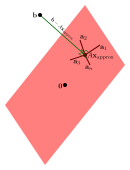
\includegraphics[width = 0.5\textwidth]{least_squares}}
\end{tabular}

\begin{align*}
\left\{\begin{array}{c}
\mathbf{a}_1 \bullet (\mathbf{b} - A\mathbf{x}_{\text{approx}}) = 0 \\
\mathbf{a}_2 \bullet (\mathbf{b} - A\mathbf{x}_{\text{approx}}) = 0 \\
\vdots \\
\mathbf{a}_n \bullet (\mathbf{b} - A\mathbf{x}_{\text{approx}}) = 0 \\
\end{array}\right. & \iff \left\{\begin{array}{c}
\mathbf{a}_1^T (\mathbf{b} - A\mathbf{x}_{\text{approx}}) = 0 \\
\mathbf{a}_2^T (\mathbf{b} - A\mathbf{x}_{\text{approx}}) = 0 \\
\vdots \\
\mathbf{a}_n^T (\mathbf{b} - A\mathbf{x}_{\text{approx}}) = 0 \\
\end{array}\right. \iff \begin{bmatrix}
\mathbf{a}_1^T \\ \mathbf{a}_2^T \\ \vdots \\ \mathbf{a}_n^T 
\end{bmatrix}(\mathbf{b} - A\mathbf{x}_{\text{approx}}) = \begin{bmatrix}
0 \\ 0 \\ \vdots \\ 0 
\end{bmatrix} \\ 
& \\
& \iff A^T(\mathbf{b} - A\mathbf{x}_{\text{approx}}) = \mathbf{0} 
\iff A^T A \mathbf{x}_{\text{approx}} = A^T \mathbf{b}
\end{align*}

The system 
\[A^T A \mathbf{x} = A^T \mathbf{b}\]
which is the {\bf normal system}, will always be consistent (will have solutions). While the solution \(\mathbf{x}\) may not be unique, the closest point \(A\mathbf{x}\) will always be unique. The solution is unique if and only if the linear mapping denoted by \(A\) is 1 to 1, which occurs if and only if the null space of \(A\) is trivial: \(\text{nullity}(A) = 0\).

\textbf{Examples:}*
\begin{itemize}
%%%%%%%%%%%%%%%%%%%%%%%%%
\item Consider the linear system:
\[\begin{bmatrix}
1 & -1 \\ 
2 & 3 \\ 
4 & 5
\end{bmatrix}\begin{bmatrix}
x_1 \\ x_2 
\end{bmatrix} = \begin{bmatrix}
2 \\ -1 \\ 5 
\end{bmatrix}\]
Attempting to directly solve this linear system yields:
\begin{align*}
\left[\begin{array}{cc|c}
1 & -1 &  2 \\ 
2 &  3 & -1 \\ 
4 &  5 &  5
\end{array}\right] 
\xrightarrow{\begin{array}{c} R_2 \rightarrow R_2 - 2R_1 \\ R_3 \rightarrow R_3 - 4R_1 \end{array}} 
\left[\begin{array}{cc|c}
1 & -1 &  2 \\ 
0 &  5 & -5 \\ 
0 &  9 & -3 
\end{array}\right] 
\xrightarrow{\begin{array}{c} R_3 \rightarrow R_3 - (9/5)R_2 \end{array}} 
\left[\begin{array}{cc|c}
1 & -1 &  2 \\ 
0 &  5 & -5 \\ 
0 &  0 &  6   
\end{array}\right] 
\end{align*}
A pivot is in the last column so the system is therefore inconsistent. A least squares solution is now what is sought. Multiplying both sides of the system on the left by \(A^T = \begin{bmatrix} 1 & 2 & 4 \\ -1 & 3 & 5 \end{bmatrix}\) gives:
\[\begin{bmatrix}
21 & 25 \\ 
25 & 35 
\end{bmatrix}\begin{bmatrix} 
x_1 \\ x_2 
\end{bmatrix} = \begin{bmatrix}
20 \\ 20
\end{bmatrix}\]
Solving this linear system gives:
\begin{align*}
\left[\begin{array}{cc|c}
21 & 25 & 20 \\ 
25 & 35 & 20
\end{array}\right] 
& \xrightarrow{\begin{array}{c} R_2 \rightarrow R_2 - (25/21)R_1 \end{array}}  
\left[\begin{array}{cc|c}
21 &        25 &        20 \\ 
  0 & 110/21 & -80/21
\end{array}\right] \\ 
& \xrightarrow{\begin{array}{c} R_2 \rightarrow (21/110)R_2 \end{array}}  
\left[\begin{array}{cc|c}
21 & 25 &      20 \\ 
  0 &   1 & -8/11
\end{array}\right] 
\xrightarrow{\begin{array}{c} R_1 \rightarrow R_1 - 25R_2 \end{array}}  
\left[\begin{array}{cc|c}
21 & 0 & 420/11 \\ 
  0 & 1 &   -8/11
\end{array}\right] \\ 
& \xrightarrow{\begin{array}{c} R_1 \rightarrow (1/21)R_1 \end{array}}  
\left[\begin{array}{cc|c}
1 & 0 & 20/11 \\ 
0 & 1 &  -8/11
\end{array}\right]
\end{align*}
The least squares solution is therefore:
\[\begin{bmatrix} 
x_1 \\ x_2 
\end{bmatrix} = \begin{bmatrix}
20/11 \\ -8/11  
\end{bmatrix}\]
%%%%%%%%%%%%%%%%%%%%%%%%%
\item Consider the linear system:
\[\begin{bmatrix}
2 & -2 \\ 
1 & 1 \\ 
3 & 1
\end{bmatrix}\begin{bmatrix}
x_1 \\ x_2 
\end{bmatrix} = \begin{bmatrix}
2 \\ -1 \\ 1 
\end{bmatrix}\]
Attempting to directly solve this linear system yields:
\begin{align*}
\left[\begin{array}{cc|c}
2 & -2 &  2 \\ 
1 &  1 & -1 \\ 
3 &  1 &  1
\end{array}\right] 
\xrightarrow{\begin{array}{c} R_2 \rightarrow R_2 - (1/2)R_1 \\ R_3 \rightarrow R_3 - (3/2)R_1 \end{array}} 
\left[\begin{array}{cc|c}
2 & -2 &  2 \\ 
0 &  2 & -2 \\ 
0 &  4 & -2 
\end{array}\right] 
\xrightarrow{\begin{array}{c} R_3 \rightarrow R_3 - 2R_2 \end{array}} 
\left[\begin{array}{cc|c}
2 & -2 &  2 \\ 
0 &  2 & -2 \\ 
0 &  0 &  2   
\end{array}\right] 
\end{align*}
A pivot is in the last column so the system is therefore inconsistent. A least squares solution is now what is sought. Multiplying both sides of the system on the left by \(A^T = \begin{bmatrix} 2 & 1 & 3 \\ -2 & 1 & 1 \end{bmatrix}\) gives:
\[\begin{bmatrix}
14 & 0 \\ 
  0 & 6 
\end{bmatrix}\begin{bmatrix} 
x_1 \\ x_2 
\end{bmatrix} = \begin{bmatrix}
6 \\ -4
\end{bmatrix}\]
Solving this linear system gives:
\begin{align*}
\left[\begin{array}{cc|c}
14 & 0 &   6 \\ 
  0 & 6 & -4
\end{array}\right] 
& \xrightarrow{\begin{array}{c} R_2 \rightarrow (1/6)R_2 \end{array}}  
\left[\begin{array}{cc|c}
14 & 0 &      6 \\ 
  0 & 1 & -2/3
\end{array}\right] \\ 
& \xrightarrow{\begin{array}{c} R_1 \rightarrow (1/14)R_1 \end{array}}  
\left[\begin{array}{cc|c}
1 & 0 &  3/7 \\ 
0 & 1 & -2/3
\end{array}\right]
\end{align*}
The least squares solution is therefore:
\[\begin{bmatrix} 
x_1 \\ x_2 
\end{bmatrix} = \begin{bmatrix}
3/7 \\ -2/3  
\end{bmatrix}\]
%%%%%%%%%%%%%%%%%%%%%%%%%
\item Consider the linear system:
\[\begin{bmatrix}
1 & 0 & -1 \\ 
2 & 1 & -2 \\ 
1 & 1 &  0 \\ 
1 & 1 & -1 
\end{bmatrix}\begin{bmatrix}
x_1 \\ x_2 \\ x_3
\end{bmatrix} = \begin{bmatrix}
6 \\ 0 \\ 9 \\ 3 
\end{bmatrix}\]
Attempting to directly solve this linear system yields:
\begin{align*}
\left[\begin{array}{ccc|c}
1 & 0 & -1 & 6 \\ 
2 & 1 & -2 & 0 \\ 
1 & 1 &  0 & 9 \\
1 & 1 & -1 & 3
\end{array}\right] 
\xrightarrow{\begin{array}{c} R_2 \rightarrow R_2 - 2R_1 \\ R_3 \rightarrow R_3 - R_1 \\ R_4 \rightarrow R_4 - R_1 \end{array}} 
\left[\begin{array}{ccc|c}
1 & 0 & -1 &    6 \\ 
0 & 1 &  0 & -12 \\ 
0 & 1 &  1 &    3 \\
0 & 1 &  0 &   -3
\end{array}\right] 
\xrightarrow{\begin{array}{c} R_3 \rightarrow R_3 - R_2 \\ R_4 \rightarrow R_4 - R_2\end{array}} 
\left[\begin{array}{ccc|c}
1 & 0 & -1 &    6 \\ 
0 & 1 &  0 & -12 \\ 
0 & 0 &  1 &  15 \\
0 & 0 &  0 &    9
\end{array}\right]  
\end{align*}
A pivot is in the last column so the system is therefore inconsistent. A least squares solution is now what is sought. Multiplying both sides of the system on the left by \(A^T = \begin{bmatrix} 1 & 2 & 1 & 1 \\ 0 & 1 & 1 & 1 \\ -1 & -2 & 0 & -1 \end{bmatrix}\) gives:
\[\begin{bmatrix}
 7 &  4 & -6 \\ 
 4 &  3 & -3 \\ 
-6 & -3 &  6  
\end{bmatrix}\begin{bmatrix} 
x_1 \\ x_2 \\ x_3
\end{bmatrix} = \begin{bmatrix}
18 \\ 12 \\ -9
\end{bmatrix}\]
Solving this linear system gives:
\begin{align*}
& \left[\begin{array}{ccc|c}
 7 &  4 & -6 & 18 \\ 
 4 &  3 & -3 & 12 \\ 
-6 & -3 &  6 & -9 
\end{array}\right] 
\xrightarrow{\begin{array}{c} R_2 \rightarrow R_2 - (4/7)R_1 \\ R_3 \rightarrow R_3 + (6/7)R_1 \end{array}}  
\left[\begin{array}{ccc|c}
7 &    4 &   -6 &     18 \\ 
0 & 5/7 & 3/7 & 12/7 \\ 
0 & 3/7 & 6/7 & 45/7 
\end{array}\right] \\ 
& \xrightarrow{\begin{array}{c} R_3 \rightarrow R_3 - (3/5)R_2 \end{array}}  
\left[\begin{array}{ccc|c}
7 &    4 &   -6 &     18 \\ 
0 & 5/7 & 3/7 & 12/7 \\ 
0 &    0 & 3/5 & 27/5 
\end{array}\right] 
\xrightarrow{\begin{array}{c} R_3 \rightarrow (5/3)R_3 \end{array}}  
\left[\begin{array}{ccc|c}
7 &    4 &   -6 &     18 \\ 
0 & 5/7 & 3/7 & 12/7 \\ 
0 &    0 &     1 &      9  
\end{array}\right] \\ 
& \xrightarrow{\begin{array}{c} R_1 \rightarrow R_1 + 6R_3 \\ R_2 \rightarrow R_2 - (3/7)R_3 \end{array}}  
\left[\begin{array}{ccc|c}
7 &    4 & 0 &      72 \\ 
0 & 5/7 & 0 & -15/7 \\ 
0 &    0 & 1 &        9  
\end{array}\right]
\xrightarrow{\begin{array}{c} R_2 \rightarrow (7/5)R_2 \end{array}}  
\left[\begin{array}{ccc|c}
7 & 4 & 0 & 72 \\ 
0 & 1 & 0 & -3 \\ 
0 & 0 & 1 &  9  
\end{array}\right] \\ 
& \xrightarrow{\begin{array}{c} R_1 \rightarrow R_1 - 4R_2 \end{array}}  
\left[\begin{array}{ccc|c}
7 & 0 & 0 & 84 \\ 
0 & 1 & 0 & -3 \\ 
0 & 0 & 1 &  9  
\end{array}\right] 
\xrightarrow{\begin{array}{c} R_1 \rightarrow (1/7)R_1 \end{array}}  
\left[\begin{array}{ccc|c}
1 & 0 & 0 & 12 \\ 
0 & 1 & 0 & -3 \\ 
0 & 0 & 1 &  9  
\end{array}\right] 
\end{align*}
The least squares solution is therefore:
\[\begin{bmatrix} 
x_1 \\ x_2 \\ x_3
\end{bmatrix} = \begin{bmatrix}
12 \\ -3 \\ 9   
\end{bmatrix}\]
\end{itemize}
*Examples from the problem set of chapter 6.4 of the textbook: \\
Anton, Howard; Rorres, Chris, \emph{Elementary Linear Algebra 11th edition, Applications Version}, Wiley, 2014.


\end{document}















